% answers.tex —— 1986 年·广东卷·理工农医类 · 参考答案与详细解析片段
% 由 tools/generate_projects.py 依来源总账自 1986/1986_数学真题_广东理_试题.md + 1986/1986_数学真题_广东理_解析正文.md + 1986/1986_数学真题_广东理_答案要点.md 生成，勿手改（改源 MD 后重跑）


\begin{gktip}
固定源为扫描 PDF，题面在 PDF 第 1—6 页，答案与解答在第 7—11 页。第 9 题的幅角主值沿用固定源选项所反映的 $[0,2\pi)$ 约定。第 12、15 题末项选项标签重复，照录但按数值判断。第 25 题的 A—E 图形选项整段缺失，不能把答案表中的字母与具体图形建立可核对映射。
\end{gktip}

\begin{answer}
\gksolhead{1}{}

\textbf{题目}：

（本题满分 50 分）本题共有 25 个小题。每一个小题都给出代号为 $A\text{、}B\text{、}C\text{、}D\text{、}E$ 的五个结论，其中只有一个结论是正确的。请把正确结论的代号选出，并在答题卷中的相应位置上涂黑（每个小题选对得 2 分，不选、选错或者选出的代号超过一个，一律得 0 分）。

（1） 通过点 $(0,2)$ 且倾斜角为 $15^\circ$ 的直线的方程是\mbox{（　　）}

（A）$y=(\sqrt3-2)x+2$　　（B）$y=(\sqrt2-1)x+2$

（C）$y=(2-\sqrt3)x+2$　　（D）$y=(\dfrac{\sqrt3}{2}-1)x+2$

（E）$y=(\sqrt3-1)x+2$

（2） 设 $\alpha,\beta\in(0,\frac\pi2)$ 且 $\operatorname{tg}\alpha=\frac43,\operatorname{tg}\beta=\frac17$，则 $\alpha-\beta=$\mbox{（　　）}

（A）$\dfrac\pi3$　　（B）$\dfrac\pi4$　　（C）$\dfrac\pi6$　　（D）$\dfrac\pi8$　　（E）$-\dfrac\pi3$

（3） 侧面为等边三角形的正三棱锥，其侧面与底面所成的二面角的余弦的值是\mbox{（　　）}

（A）$\dfrac{\sqrt3}{2}$　　（B）$\dfrac{\sqrt2}{2}$　　（C）$\dfrac12$　　（D）$\dfrac13$　　（E）$\dfrac{\sqrt2}{3}$

\Needspace{5\baselineskip}
（4） 参数方程

\nopagebreak[4]
\[
\begin{cases}
x=1-2\sin\varphi,\\
y=\cos\varphi
\end{cases}
\qquad(\varphi\text{ \text{为参数}})
\]

所表示的曲线是\mbox{（　　）}

（A）圆　　（B）焦点在 $x$ 轴上的双曲线　　（C）焦点在 $y$ 轴上的双曲线

（D）焦点在 $x$ 轴上的椭圆　　（E）焦点在 $y$ 轴上的椭圆

（5） 复数 $\sin95^\circ+i\cos95^\circ$ 的一个辐角是\mbox{（　　）}

（A）$-85^\circ$　　（B）$-5^\circ$　　（C）$5^\circ$　　（D）$85^\circ$　　（E）$95^\circ$

（6） 若复数 $(\sqrt3+i)^n$ 是一个纯虚数，则 $n$ 的一个可能的值是\mbox{（　　）}

（A）5　　（B）6　　（C）7　　（D）8　　（E）9

（7） 在复平面上，设动点 $Z$ 对应的复数为 $z$，$Z$ 到复数 $-i$ 和 $1+i$ 所对应的点的距离之和等于 5，则动点 $Z$ 的轨迹方程是\mbox{（　　）}

（A）$|z+i|+|z-1-i|=5$　　（B）$|z-i|+|z+1+i|=5$

（C）$(z+i)+(z-1-i)=5$　　（D）$(z-i)+(z+1+i)=5$

（E）$(z+i)^2+(z-1-i)^2=25$

（8） 要从 8 名男医生和 7 名女医生中选 5 人组成一个医疗小组，如果医疗小组中至少有 2 名男医生和至少有 2 名女医生，则不同选法的种数是\mbox{（　　）}

（A）$(C_8^3+C_7^2)\square(C_7^3+C_8^2)$

（B）$(C_8^3+C_7^2)+(C_7^3+C_8^2)$

（C）$C_8^2\square C_7^3$　　（D）$C_8^2\square C_7^2\square C_{11}^1$

（E）$C_8^2\square C_7^3+C_8^3\square C_7^2$

（9） 要排一张有 5 个独唱节目和 3 个合唱节目的演出节目表，如果合唱节目不排头，并且任何两个合唱节目不相邻，则不同排法的种数是\mbox{（　　）}

（A）$P_8^8$　　（B）$P_5^5\square P_3^3$　　（C）$P_5^5\square P_5^3$

（D）$P_5^5\square P_8^3$　　（E）$P_8^5\square P_8^3$

（10） 设 $a,b$ 为实数且 $a+b=3$，则 $2^a+2^b$ 的最小值是\mbox{（　　）}

（A）6　　（B）$4\sqrt2$　　（C）$2\sqrt2$　　（D）$2\sqrt6$　　（E）8

\Needspace{5\baselineskip}
（11） 若 $\operatorname{ctg}\theta=3$，则

\nopagebreak[4]
\[
\cos^2\theta+\frac12\sin2\theta
\]

的值是\mbox{（　　）}

（A）$-\dfrac65$　　（B）$-\dfrac45$　　（C）$\dfrac45$　　（D）1　　（E）$\dfrac65$

\Needspace{5\baselineskip}
（12） 若 $\theta\in(\frac{5\pi}4,\frac{3\pi}2)$，则

\nopagebreak[4]
\[
\sqrt{1-\sin2\theta}
\]

等于\mbox{（　　）}

（A）$\cos\theta-\sin\theta$　　（B）$\sin\theta+\cos\theta$

（C）$\sin\theta-\cos\theta$　　（D）$-\cos\theta-\sin\theta$

（D）$|\cos\theta|-|\sin\theta|$

\Needspace{5\baselineskip}
（13） 函数

\nopagebreak[4]
\[
y=\cos x-\sin^2x-\cos2x+\frac74
\]

的最大值是\mbox{（　　）}

（A）$\dfrac74$　　（B）2　　（C）$\dfrac94$　　（D）$\dfrac{17}4$　　（E）$\dfrac{19}4$

\Needspace{5\baselineskip}
（14） 计算下式：

\nopagebreak[4]
\[
\operatorname{arctg}(1-\sqrt2)
\]

等于\mbox{（　　）}

（A）$-\dfrac{5\pi}8$　　（B）$-\dfrac{3\pi}8$　　（C）$-\dfrac\pi8$

（D）$\dfrac\pi8$　　（E）$\dfrac{3\pi}8$

\Needspace{5\baselineskip}
（15） 椭圆

\nopagebreak[4]
\[
\frac{(x+1)^2}{4}+y^2=1
\]

\Needspace{5\baselineskip}
与抛物线

\nopagebreak[4]
\[
y=1-(x+1)^2
\]

的交点的个数是\mbox{（　　）}

（A）0　　（B）1　　（C）2　　（D）3　　（D）4

\Needspace{5\baselineskip}
（16） 若动圆与圆

\nopagebreak[4]
\[
(x+2)^2+y^2=4
\]

相外切且与直线 $x=2$ 相切，则动圆的圆心的轨迹方程是\mbox{（　　）}

（A）$y^2-12x+12=0$　　（B）$y^2+12x-12=0$　　（C）$y^2+8x=0$

（D）$y^2-8x=0$　　（E）$y^2-6x+6=0$

\Needspace{5\baselineskip}
（17） 通过点 $A(3,4)$ 及双曲线

\nopagebreak[4]
\[
\frac{x^2}{6}-\frac{y^2}{3}=1
\]

的两个焦点的圆的方程是\mbox{（　　）}

（A）$x^2+(y-\frac83)^2=\frac{145}{9}$　　（B）$(x-\frac83)^2+y^2=\frac{145}{9}$

（C）$(x-2)^2+y^2=13$　　（D）$x^2+(y-2)^2=13$　　（E）$x^2+(y-\frac{11}4)^2=\frac{169}{16}$

\Needspace{5\baselineskip}
（18） 函数

\nopagebreak[4]
\[
y=\sqrt{x^2+2x-3}
\]

的单调下降区间是\mbox{（　　）}

（A）$(-\infty,-3]$　　（B）$[-3,+\infty)$　　（C）$(-\infty,-1]$

（D）$[-1,+\infty)$　　（E）$[-3,-1]$

\Needspace{5\baselineskip}
（19） 函数

\nopagebreak[4]
\[
y=\log_{\cos1}(\cos x)
\]

的值域是\mbox{（　　）}

（A）$[-1,1]$　　（B）$(-\infty,+\infty)$　　（C）$(-\infty,0]$

（D）$[0,+\infty)$　　（E）$[\cos1,(\cos1)^{-1}]$

（20） 在空间中，下列命题中成立的是\mbox{（　　）}

（A）过平面 $\alpha$ 外的两点，必有且只有一个平面与平面 $\alpha$ 垂直。

（B）若直线 $l$ 上有两点到平面 $\alpha$ 的距离相等，则直线 $l$ 必平行于平面 $\alpha$。

（C）若直线 $l$ 与平面 $\alpha$ 内的无数多条直线垂直，则直线 $l$ 必垂直于平面 $\alpha$。

（D）互相平行的两条直线在一个平面内的射影必然是互相平行的两条直线。

（E）若点 $P$ 到三角形的三条边的距离相等，则点 $P$ 在该三角形所在平面内的射影必然是三角形的内心。

（21） 四棱锥成为正四棱锥的一个充分但不必要的条件是\mbox{（　　）}

（A）各侧面是等边三角形　　（B）底面是正方形

（C）各侧面三角形的顶角是 $45^\circ$　　（D）各侧面是等腰三角形且底面为正方形

（E）顶点到底面的射影在底面四边形对角线的交点上

\Needspace{5\baselineskip}
（22） 设有函数

\nopagebreak[4]
\[
\text{① }y=\cos\frac{x+3\pi}{2},\qquad
\text{② }y=\sin\frac{x+5\pi}{2},
\]

则\mbox{（　　）}

（A）①与②都是奇函数　　（B）①与②都是偶函数

（C）①是奇函数而②是偶函数　　（D）①是偶函数而②是奇函数

（E）①与②中至少有一个既不是奇函数也不是偶函数

\Needspace{5\baselineskip}
（23） 设函数

\nopagebreak[4]
\[
y=\operatorname{tg}(\operatorname{arctg}\,2x),\qquad
y=\operatorname{arctg}(\operatorname{tg}\,2x),
\]

\Needspace{5\baselineskip}
与

\nopagebreak[4]
\[
y=\sin(\arcsin 2x)
\]

的图象分别记为 $l_1,l_2,l_3$，则\mbox{（　　）}

（A）$l_1,l_2,l_3$ 都相同　　（B）只有 $l_1$ 与 $l_2$ 相同

（C）只有 $l_1$ 与 $l_3$ 相同　　（D）只有 $l_2$ 与 $l_3$ 相同

（E）$l_1,l_2,l_3$ 都不相同

（24） 若点 $A$ 的坐标为 $(3,2)$，$F$ 为抛物线 $y^2=2x$ 的焦点，点 $P$ 在该抛物线上移动，为使 $|PA|+|PF|$ 取最小值，点 $P$ 的坐标应为\mbox{（　　）}

（A）$(0,0)$　　（B）$(1,1)$　　（C）$(2,2)$　　（D）$(\frac12,1)$　　（E）$(1,\sqrt2)$

\Needspace{5\baselineskip}
（25） 若函数 $y=f(x)$ 是函数

\nopagebreak[4]
\[
y=1-\sqrt{1-x^2},\qquad -1\le x\le0
\]

的反函数，则 $y=f(x)$ 的图象大致形状是\mbox{（　　）}

\begin{gktip}
固定源第 4 页题干之后的 A—E 图形选项区域完全空白。本文只保留题干和固定源答案表记录，不凭空补画图形。
\end{gktip}

\Needspace{4\baselineskip}
\textbf{解析}

\gksubpart{（1）}

\Needspace{5\baselineskip}
令 $t=2^x>0$，则

\nopagebreak[4]
\[
2t^2-9t+4=(2t-1)(t-4)=0.
\]

故 $t=\frac12$ 或 $4$，得到 $x=-1,2$。

\gksubpart{（2）}

\Needspace{5\baselineskip}
斜率为 $\tan15^\circ=2-\sqrt3$，所以过 $(0,2)$ 的直线为

\nopagebreak[4]
\[
y=(2-\sqrt3)x+2.
\]

\gksubpart{（3）}

\Needspace{5\baselineskip}
第二条直线除以 2 得 $3x+4y+3=0$，所以两平行线距离为

\nopagebreak[4]
\[
\frac{|(-12)-3|}{\sqrt{3^2+4^2}}=3.
\]

\gksubpart{（4）}

\nopagebreak[4]
\[
x^2+2x-y^2+2y
=(x+1)^2-(y-1)^2.
\]

\Needspace{5\baselineskip}
所以曲线是

\nopagebreak[4]
\[
x-y+2=0,\qquad x+y=0,
\]

两直线互相垂直。

\gksubpart{（5）}

\nopagebreak[4]
\[
\sin^2\alpha=\frac{1-\cos2\alpha}{2}
=\frac45.
\]

\Needspace{5\baselineskip}
由于 $\alpha\in[0,\frac\pi2]$，故

\nopagebreak[4]
\[
\sin\alpha=\frac{2\sqrt5}{5}.
\]

\gksubpart{（6）}

\nopagebreak[4]
\[
P_m^3=m(m-1)(m-2),\qquad
6C_m^4=\frac{m(m-1)(m-2)(m-3)}4.
\]

约去公共因子得 $m-3=4$，所以 $m=7$。

\gksubpart{（7）}

\Needspace{5\baselineskip}
函数 $y=\log_{\frac12}x$ 在 $(0,8]$ 上递减，且

\nopagebreak[4]
\[
\log_{\frac12}8=-3,\qquad
\lim_{x\to0^+}\log_{\frac12}x=+\infty.
\]

故值域为 $[-3,+\infty)$。

\gksubpart{（8）}

\nopagebreak[4]
\[
A=(-1,3),\qquad
B=(-\infty,0)\cup(2,+\infty),
\]

\Needspace{5\baselineskip}
因此

\nopagebreak[4]
\[
A\cap B=(-1,0)\cup(2,3).
\]

\gksubpart{（9）}

\Needspace{5\baselineskip}
性别构成只能是 2 男 3 女或 3 男 2 女，故选法数为

\nopagebreak[4]
\[
C_8^2C_7^3+C_8^3C_7^2.
\]

\gksubpart{（10）}

\Needspace{5\baselineskip}
因 $-x^2-1<0$ 恒成立，原不等式等价于

\nopagebreak[4]
\[
x^2-x-6<0
\Longleftrightarrow
(x-3)(x+2)<0.
\]

故 $-2<x<3$。

\gksubpart{（11）}

\nopagebreak[4]
\[
\sin95^\circ+i\cos95^\circ
=\cos(-5^\circ)+i\sin(-5^\circ),
\]

所以一个辐角为 $-5^\circ$。

\gksubpart{（12）}

\Needspace{5\baselineskip}
正三棱锥侧面高为 $\frac{\sqrt3}{2}a$，底面中心到一边的距离为 $\frac{\sqrt3}{6}a$，故二面角余弦为

\nopagebreak[4]
\[
\frac{\sqrt3 a/6}{\sqrt3 a/2}=\frac13.
\]

\gksubpart{（13）}

\Needspace{5\baselineskip}
圆台高为

\nopagebreak[4]
\[
h=\sqrt{(3\sqrt2)^2-(4-1)^2}=3.
\]

\Needspace{5\baselineskip}
体积为

\nopagebreak[4]
\[
\frac13\pi h(4^2+4\cdot1+1^2)=21\pi.
\]

\gksubpart{（14）}

\Needspace{5\baselineskip}
按题面无度数符号的通常约定取弧度。因为 $0<1<\frac\pi2$，在该区间内

\nopagebreak[4]
\[
\cos1<\sin1<\tan1.
\]

\gksubpart{（15）}

\nopagebreak[4]
\[
\tan(\alpha+\beta)
=\frac{\frac17+\frac34}{1-\frac17\cdot\frac34}=1.
\]

且 $\alpha+\beta\in(0,\frac\pi2)$，所以 $\alpha+\beta=\frac\pi4$。

\gksubpart{（16）}

\nopagebreak[4]
\[
1+\sin2\theta-\cos2\theta
=2\sin\theta(\sin\theta+\cos\theta),
\]

\nopagebreak[4]
\[
1+\sin2\theta+\cos2\theta
=2\cos\theta(\sin\theta+\cos\theta).
\]

比值为 $\tan\theta$。

\gksubpart{（17）}

\nopagebreak[4]
\[
\sqrt{1-\cos^2\beta}=|\sin\beta|,
\qquad
\sqrt{1-\sin^2\beta}=|\cos\beta|.
\]

等式右端为 $\sin\beta-\cos\beta$，恰在 $\beta\in[\frac\pi2,\pi]$ 时与左端相同。

\gksubpart{（18）}

\nopagebreak[4]
\[
\operatorname{ctg}\frac{9\pi}{8}
=\operatorname{ctg}\frac\pi8
=\sqrt2+1.
\]

\gksubpart{（19）}

\nopagebreak[4]
\[
\begin{aligned}
y&=-2(1-\sin^2x)-2\sin x+\frac92\\
&=2\left(\sin x-\frac12\right)^2+2.
\end{aligned}
\]

最小值为 $2$。

\gksubpart{（20）}

\Needspace{5\baselineskip}
令 $u=(x+1)^2$，则

\nopagebreak[4]
\[
\frac u4+(1-u)^2=1
\Longleftrightarrow
u\left(u-\frac74\right)=0.
\]

$u=0$ 给出 1 个交点，$u=\frac74$ 给出 2 个交点，共 3 个。

\gksubpart{（21）}

\Needspace{5\baselineskip}
设动圆圆心为 $(x,y)$，由外切条件

\nopagebreak[4]
\[
\sqrt{(x+2)^2+y^2}=|x-2|+2.
\]

\Needspace{5\baselineskip}
可行支为 $x<2$，平方化简得

\nopagebreak[4]
\[
y^2+12x-12=0.
\]

\gksubpart{（22）}

\Needspace{5\baselineskip}
椭圆焦点为 $(-1,0),(1,0)$。过两个焦点的圆心设为 $(0,k)$，其半径平方为 $1+k^2$。代入点 $(3,4)$：

\nopagebreak[4]
\[
9+(4-k)^2=1+k^2,
\]

\Needspace{5\baselineskip}
得 $k=2$，故圆方程为

\nopagebreak[4]
\[
x^2+(y-2)^2=13.
\]

\gksubpart{（23）}

\Needspace{5\baselineskip}
定义域为

\nopagebreak[4]
\[
(-\infty,-3]\cup[1,+\infty),
\]

\Needspace{5\baselineskip}
且

\nopagebreak[4]
\[
y'=\frac{x+1}{\sqrt{x^2+2x-3}}.
\]

在 $(-\infty,-3]$ 上导数为负，在 $[1,+\infty)$ 上导数为正，下降区间为 $(-\infty,-3]$。

\gksubpart{（24）}

\Needspace{5\baselineskip}
令抛物线上的点为 $P=(\frac{t^2}{2},t)$，焦点为 $F=(\frac12,0)$。有

\nopagebreak[4]
\[
PF=\frac{t^2+1}{2}.
\]

\Needspace{5\baselineskip}
当 $t^2<6$ 时，

\nopagebreak[4]
\[
PA^2-\left(3-\frac{t^2}{2}\right)^2=(t-2)^2\ge0,
\]

从而 $PA+PF\ge\frac72$；当 $t^2\ge6$ 时 $PF\ge\frac72$。等号在 $t=2$ 取得，故 $P=(2,2)$。

\gksubpart{（25）}

\Needspace{5\baselineskip}
由反函数关系交换 $x,y$：

\nopagebreak[4]
\[
x=1-\sqrt{1-y^2},\qquad 0\le y\le1.
\]

\Needspace{5\baselineskip}
于是

\nopagebreak[4]
\[
y^2=2x-x^2,\qquad 0\le x\le1,\qquad y\le0.
\]

图象是圆 $(x-1)^2+y^2=1$ 的左下四分之一弧，从 $(0,0)$ 到 $(1,-1)$。固定源中该题图形选项区域为空白，答案表的（E）无法与具体图形作视觉核对。

\gkanswer{答案（1）：C}

\gkanswer{答案（2）：B}

\gkanswer{答案（3）：D}

\gkanswer{答案（4）：D}

\gkanswer{答案（5）：B}

\gkanswer{答案（6）：E}

\gkanswer{答案（7）：A}

\gkanswer{答案（8）：E}

\gkanswer{答案（9）：C}

\gkanswer{答案（10）：B}

\gkanswer{答案（11）：E}

\gkanswer{答案（12）：A}

\gkanswer{答案（13）：B}

\gkanswer{答案（14）：C}

\gkanswer{答案（15）：D（固定源末两项均印 D）}

\gkanswer{答案（16）：B}

\gkanswer{答案（17）：D}

\gkanswer{答案（18）：A}

\gkanswer{答案（19）：D}

\gkanswer{答案（20）：E}

\gkanswer{答案（21）：A}

\gkanswer{答案（22）：C}

\gkanswer{答案（23）：E}

\gkanswer{答案（24）：C}

\gkanswer{答案（25）：E（固定源图形选项缺失）}

\end{answer}
\begin{answer}
\gksolhead{2}{}

\textbf{题目}：

（本题满分 30 分）本题共有 10 个小题，每一个小题满分 3 分，只要求直接写出结果。

\Needspace{5\baselineskip}
（1） 函数

\nopagebreak[4]
\[
y=2\log_3x\qquad(x>0)
\]

的反函数是 $\underline{\hspace{2em}}$。

\Needspace{5\baselineskip}
（2） 将极坐标方程

\nopagebreak[4]
\[
\rho=\operatorname{tg}\theta\ \square\ \sec\theta
\]

化为直角坐标方程，得 $\underline{\hspace{2em}}$。

\begin{gktip}
固定源中的乘法位置显示为方框缺字形 $\square$，按题意解释为乘法，但题面记录不替换该字形。
\end{gktip}

\Needspace{5\baselineskip}
（3） 若球内切于圆柱，则它们的表面积之比

\nopagebreak[4]
\[
S_{\text{\text{圆柱全}}}:S_{\text{\text{球}}}
\]

的值是 $\underline{\hspace{2em}}$。

\Needspace{5\baselineskip}
（4） 中心在原点的双曲线，若其实半轴长为 2，一条准线的方程为

\nopagebreak[4]
\[
x=-\frac12,
\]

则该双曲线的离心率的值是 $\underline{\hspace{2em}}$。

\Needspace{5\baselineskip}
（5） 设函数 $y=\lg(x^2-x-2)$ 的定义域为 $A$，函数

\nopagebreak[4]
\[
y=\sqrt{\frac{x+2}{1-x}}
\]

的定义域为 $B$，则 $A\cap B=$ $\underline{\hspace{2em}}$。

\Needspace{5\baselineskip}
（6） 已知等差数列 $\{a_n\}$ 的公差是正数，且

\nopagebreak[4]
\[
a_3a_7=-12,\qquad a_4+a_6=-4,
\]

则前 20 项的和 $S_{20}=$ $\underline{\hspace{2em}}$。

\Needspace{5\baselineskip}
（7） 计算下式：

\nopagebreak[4]
\[
(2x-1)^5
\]

的展开式中各项系数的绝对值的和为 $\underline{\hspace{2em}}$。

\Needspace{5\baselineskip}
（8） 求极限：

\nopagebreak[4]
\[
\lim_{n\to\infty}\sqrt n\left(\sqrt{n+1}-\sqrt n\right)
=\underline{\hspace{2em}}\text{。}
\]

\Needspace{5\baselineskip}
（9） 方程

\nopagebreak[4]
\[
\sin\left(\frac\pi3-x\right)\ \square\
\cos\left(x+\frac\pi3\right)-\frac{\sqrt3}{2}=0
\]

的解集是 $\underline{\hspace{2em}}$。

\begin{gktip}
固定源中两个三角函数之间的乘法位置显示为方框缺字形 $\square$，按题意解释为乘法，但题面记录不替换该字形。
\end{gktip}

\Needspace{5\baselineskip}
（10） 当 $a$ 在 $(-\infty,0)$ 内变化时，要使过三点

\nopagebreak[4]
\[
O(0,0),\qquad A(-4,0),\qquad B(-2,a)
\]

的圆的圆心在 $\triangle AOB$ 内（包括边界），则 $a$ 允许取的最大值是 $\underline{\hspace{2em}}$。

\Needspace{4\baselineskip}
\textbf{解析}

\gksubpart{（1）}

\nopagebreak[4]
\[
y=2\log_3x
\Longleftrightarrow
x=3^{y/2},
\]

故反函数为 $y=3^{x/2}=(\sqrt3)^x$。

\gksubpart{（2）}

\Needspace{5\baselineskip}
按固定源乘法缺字解释，

\nopagebreak[4]
\[
\rho=\tan\theta\sec\theta
=\frac{\sin\theta}{\cos^2\theta}.
\]

\Needspace{5\baselineskip}
利用 $x=\rho\cos\theta,\ y=\rho\sin\theta$，得

\nopagebreak[4]
\[
\rho\cos^2\theta=\sin\theta
\Longrightarrow x^2=y.
\]

\gksubpart{（3）}

\Needspace{5\baselineskip}
设球半径为 $r$，内切圆柱高为 $2r$。则

\nopagebreak[4]
\[
S_{\text{\text{圆柱全}}}=6\pi r^2,\qquad
S_{\text{\text{球}}}=4\pi r^2,
\]

比值为 $\frac32$。

\gksubpart{（4）}

\Needspace{5\baselineskip}
双曲线准线为 $x=\pm a/e$，由 $a=2$、准线 $x=-\frac12$ 得

\nopagebreak[4]
\[
\frac2e=\frac12,\qquad e=4.
\]

\gksubpart{（5）}

\nopagebreak[4]
\[
A=(-\infty,-1)\cup(2,+\infty),
\qquad
B=[-2,1),
\]

\Needspace{5\baselineskip}
故

\nopagebreak[4]
\[
A\cap B=[-2,-1).
\]

\gksubpart{（6）}

\Needspace{5\baselineskip}
令 $a_5=\frac{a_4+a_6}{2}=-2$，设公差为 $d>0$，则

\nopagebreak[4]
\[
a_3=-2-2d,\qquad a_7=-2+2d.
\]

\Needspace{5\baselineskip}
由 $a_3a_7=-12$ 得 $d=2$，进而 $a_1=-10$，所以

\nopagebreak[4]
\[
S_{20}=10(2a_1+19d)=180.
\]

\gksubpart{（7）}

\Needspace{5\baselineskip}
逐项取绝对值等价于把二项式中的减号改为加号，因此

\nopagebreak[4]
\[
\sum|\text{\text{各项系数}}|=(2+1)^5=243.
\]

\gksubpart{（8）}

\nopagebreak[4]
\[
\sqrt n(\sqrt{n+1}-\sqrt n)
=\frac{\sqrt n}{\sqrt{n+1}+\sqrt n}
=\frac1{\sqrt{1+1/n}+1}
\longrightarrow\frac12.
\]

\gksubpart{（9）}

\Needspace{5\baselineskip}
按固定源乘法缺字解释，原方程为

\nopagebreak[4]
\[
\sin\left(\frac\pi3-x\right)
\cos\left(x+\frac\pi3\right)
-\frac{\sqrt3}{2}=0.
\]

\Needspace{5\baselineskip}
积化和差得

\nopagebreak[4]
\[
\sin\left(\frac\pi3-x\right)
\cos\left(x+\frac\pi3\right)
=\frac{\sqrt3}{4}-\frac12\sin2x.
\]

\Needspace{5\baselineskip}
所以 $\sin2x=-\frac{\sqrt3}{2}$，解集为

\nopagebreak[4]
\[
x=k\pi+\frac{2\pi}{3}
\quad\text{\text{或}}\quad
x=k\pi+\frac{5\pi}{6},
\qquad k\in\mathbb Z.
\]

\gksubpart{（10）}

\Needspace{5\baselineskip}
设圆心为 $(-2,k)$。由到 $O$ 与 $B$ 等距：

\nopagebreak[4]
\[
4+k^2=(a-k)^2,
\qquad
k=\frac{a^2-4}{2a}.
\]

圆心在线段 $x=-2$ 的三角形内部等价于 $a\le k\le0$。在 $a<0$ 下，$k\le0$ 等价于 $a\le-2$，所以最大值为 $-2$。

\gkanswer{答案（1）：$y=(\sqrt3)^x$}

\gkanswer{答案（2）：$x^2=y$（固定源乘号为缺字方框）}

\gkanswer{答案（3）：$\dfrac32$}

\gkanswer{答案（4）：$4$}

\gkanswer{答案（5）：$[-2,-1)$}

\gkanswer{答案（6）：$180$}

\gkanswer{答案（7）：$243$}

\gkanswer{答案（8）：$\dfrac12$}

\gkanswer{答案（9）：$\displaystyle x=k\pi+\frac{2\pi}{3}\text{ \text{或} }x=k\pi+\frac{5\pi}{6},\ k\in\mathbb Z$}

\gkanswer{答案（10）：$-2$}

\end{answer}
\begin{answer}
\gksolhead{3}{}

\textbf{题目}：

\Needspace{5\baselineskip}
（本题满分 8 分）设有对数方程

\nopagebreak[4]
\[
\lg(ax)=2\lg(x-1).
\]

（1） 当 $a=2$ 时，解该对数方程；

（2） 证明：当 $a>0$ 时，该对数方程有且只有一个解，并求出它的解。

\Needspace{4\baselineskip}
\textbf{解析}

\gksubpart{（1）}

\Needspace{5\baselineskip}
对 $0<x-1$ 且 $ax>0$，当 $a=2$ 时

\nopagebreak[4]
\[
\lg(2x)=2\lg(x-1)
\Longleftrightarrow
2x=(x-1)^2.
\]

解得 $x=2\pm\sqrt3$，由 $x>1$ 保留 $x=2+\sqrt3$。

\gksubpart{（2）}

\Needspace{5\baselineskip}
一般地

\nopagebreak[4]
\[
\lg(ax)=2\lg(x-1)
\Longleftrightarrow
x^2-(a+2)x+1=0.
\]

\Needspace{5\baselineskip}
定义域迫使 $a>0$、$x>1$。当 $a>0$ 时，判别式 $a^2+4a>0$，两根为

\nopagebreak[4]
\[
x_\pm=\frac{a+2\pm\sqrt{a^2+4a}}2.
\]

\Needspace{5\baselineskip}
其中 $x_+-1>0$、$x_--1<0$，所以恰有一个合法解：

\nopagebreak[4]
\[
x=\frac{a+2+\sqrt{a^2+4a}}2.
\]

有解的参数范围为 $a>0$。

\gkanswer{答案（1）：$x=2+\sqrt3$}

\gkanswer{答案（2）：$a>0$，且唯一解为 $\displaystyle x=\frac{a+2+\sqrt{a^2+4a}}2$}

\end{answer}
\begin{answer}
\gksolhead{4}{}

\textbf{题目}：

（本题满分 12 分）在三棱锥 $S-ABC$ 中，平面 $SAC\perp ABC$，$AB=AC=a$，$\angle BAC=90^\circ$，$SA=SC=b$。求：

（1） 棱 $SB$ 与平面 $ABC$ 所成角的正切；

（2） 三棱锥被过 $S$ 且与 $BC$ 垂直的平面所截得的截面面积。
\nopagebreak[4]
\begin{center}% 1986 年广东卷理工农医类第 4 题：三棱锥
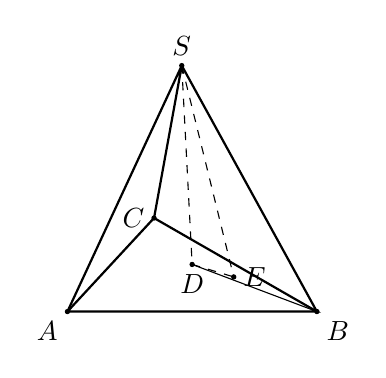
\begin{tikzpicture}[scale=0.88,>=stealth]
  \coordinate (A) at (0,0);
  \coordinate (B) at (3.6,0);
  \coordinate (C) at (1.25,1.35);
  \coordinate (S) at (1.65,3.55);
  \coordinate (D) at (1.8,0.68);
  \coordinate (E) at (2.4,0.5);

  \draw[thick] (A)--(B)--(C)--cycle;
  \draw[thick] (S)--(A) (S)--(B) (S)--(C);
  \draw[dashed] (A)--(C);
  \draw[dashed] (S)--(D) (S)--(E) (D)--(E);
  \draw (D)--(B);
  \fill (A) circle (1.1pt) node[below left] {$A$};
  \fill (B) circle (1.1pt) node[below right] {$B$};
  \fill (C) circle (1.1pt) node[left] {$C$};
  \fill (S) circle (1.1pt) node[above] {$S$};
  \fill (D) circle (1.1pt) node[below] {$D$};
  \fill (E) circle (1.1pt) node[right] {$E$};
\end{tikzpicture}
\end{center}
\nopagebreak[4]
\Needspace{4\baselineskip}
\textbf{解析}

\gksubpart{（1）}

\Needspace{5\baselineskip}
在三棱锥中，于平面 $SAC$ 内作 $SD\perp AC$。由 $SA=SC=b$，$D$ 是 $AC$ 中点，故

\nopagebreak[4]
\[
SD=\sqrt{b^2-\frac{a^2}{4}}.
\]

\Needspace{5\baselineskip}
又因 $SAC\perp ABC$，所以 $SD\perp ABC$。在底面中

\nopagebreak[4]
\[
BD=\sqrt{a^2+\left(\frac a2\right)^2}
=\frac{\sqrt5}{2}a.
\]

\Needspace{5\baselineskip}
因此棱 $SB$ 与底面所成角的正切为

\nopagebreak[4]
\[
\frac{SD}{BD}
=\frac{\sqrt{20b^2-5a^2}}{5a}.
\]

\gksubpart{（2）}

\Needspace{5\baselineskip}
再在平面 $SBC$ 内作 $SE\perp BC$。截面为三角形 $SDE$，且

\nopagebreak[4]
\[
DE=\frac{\sqrt2}{4}a,\qquad SD\perp DE.
\]

\Needspace{5\baselineskip}
所以截面面积为

\nopagebreak[4]
\[
\frac12SD\cdot DE
=\frac a{16}\sqrt{8b^2-2a^2}.
\]

\gkanswer{答案（1）：$\displaystyle \frac{\sqrt{20b^2-5a^2}}{5a}$}

\gkanswer{答案（2）：$\displaystyle \frac a{16}\sqrt{8b^2-2a^2}$}

\end{answer}
\begin{answer}
\gksolhead{5}{}

\textbf{题目}：

\Needspace{5\baselineskip}
（本题满分 12 分）设

\nopagebreak[4]
\[
a_n=\cos n\alpha,\qquad 0<\alpha<\pi.
\]

（1） 试用 $a_{n-1},a_{n-2}$ 表示 $a_n$；

\Needspace{5\baselineskip}
（2） 用数学归纳法证明

\nopagebreak[4]
\[
a_1+a_2+\cdots+a_n
=\frac{\sin\frac{n\alpha}{2}\cos\frac{(n+1)\alpha}{2}}
{\sin\frac\alpha2};
\]

\Needspace{5\baselineskip}
（3） 求

\nopagebreak[4]
\[
a_1-a_2+a_3-a_4+\cdots+(-1)^{k+1}a_k+\cdots-a_{2n}+a_{2n+1}.
\]

\Needspace{4\baselineskip}
\textbf{解析}

\gksubpart{（1）}

\Needspace{5\baselineskip}
由

\nopagebreak[4]
\[
a_n=\cos n\alpha
\]

\Needspace{5\baselineskip}
和余弦和差公式，

\nopagebreak[4]
\[
a_n+a_{n-2}
=2\cos(n-1)\alpha\cos\alpha
=2a_{n-1}\cos\alpha.
\]

\Needspace{5\baselineskip}
故

\nopagebreak[4]
\[
a_n=2a_{n-1}\cos\alpha-a_{n-2}.
\]

\gksubpart{（2）}

\Needspace{5\baselineskip}
设

\nopagebreak[4]
\[
S_n=a_1+a_2+\cdots+a_n.
\]

\Needspace{5\baselineskip}
当 $n=1$ 时公式成立。若对 $n=k$ 成立，则

\nopagebreak[4]
\[
S_{k+1}=S_k+\cos(k+1)\alpha.
\]

\Needspace{5\baselineskip}
使用积化和差整理，得到

\nopagebreak[4]
\[
S_{k+1}
=\frac{\sin\frac{(k+1)\alpha}{2}
\cos\frac{(k+2)\alpha}{2}}
{\sin\frac\alpha2}.
\]

\Needspace{5\baselineskip}
因此由数学归纳法

\nopagebreak[4]
\[
a_1+\cdots+a_n
=\frac{\sin\frac{n\alpha}{2}
\cos\frac{(n+1)\alpha}{2}}
{\sin\frac\alpha2}.
\]

\gksubpart{（3）}

\Needspace{5\baselineskip}
设交错和为

\nopagebreak[4]
\[
T=\sum_{j=1}^{2n+1}(-1)^{j+1}\cos(j\alpha).
\]

\Needspace{5\baselineskip}
利用复数等比数列，

\nopagebreak[4]
\[
\sum_{j=1}^{2n+1}(-1)^{j+1}e^{ij\alpha}
=e^{i(n+1)\alpha}
\frac{\cos\frac{(2n+1)\alpha}{2}}
{\cos\frac\alpha2}.
\]

\Needspace{5\baselineskip}
取实部得

\nopagebreak[4]
\[
T=\frac{\cos((n+1)\alpha)
\cos\frac{(2n+1)\alpha}{2}}
{\cos\frac\alpha2}.
\]

\gkanswer{答案（1）：$\displaystyle a_n=2a_{n-1}\cos\alpha-a_{n-2}$}

\gkanswer{答案（2）：见解析正文。}

\gkanswer{答案（3）：$\displaystyle \frac{\cos((n+1)\alpha)\cos\frac{(2n+1)\alpha}{2}}{\cos\frac\alpha2}$}

\end{answer}
\begin{answer}
\gksolhead{6}{}

\textbf{题目}：

\Needspace{5\baselineskip}
（本题满分 12 分）已知椭圆 $C$ 的直角坐标方程为

\nopagebreak[4]
\[
\frac{x^2}{4}+\frac{y^2}{3}=1,
\]

\Needspace{5\baselineskip}
试确定 $m$ 的取值范围，使得对于直线

\nopagebreak[4]
\[
y=4x+m,
\]

椭圆 $C$ 上有不同的两点关于该直线对称。

\Needspace{4\baselineskip}
\textbf{解析}

\Needspace{5\baselineskip}
若弦所在直线为

\nopagebreak[4]
\[
y=-\frac x4+n,
\]

\Needspace{5\baselineskip}
与椭圆联立，交点为两个不同点的条件是

\nopagebreak[4]
\[
n^2<\frac{13}{4}.
\]

\Needspace{5\baselineskip}
由韦达定理，弦中点为

\nopagebreak[4]
\[
M=\left(\frac{4n}{13},\frac{12n}{13}\right).
\]

\Needspace{5\baselineskip}
因 $M$ 在 $y=4x+m$ 上，

\nopagebreak[4]
\[
\frac{12n}{13}
=4\cdot\frac{4n}{13}+m,
\qquad
m=-\frac{4n}{13}.
\]

\Needspace{5\baselineskip}
于是

\nopagebreak[4]
\[
-\frac{2\sqrt{13}}{13}
<m<
\frac{2\sqrt{13}}{13}.
\]

端点对应相切，只得到一个交点，不能取等号。

\gkanswer{答案：$\displaystyle -\frac{2\sqrt{13}}{13}<m<\frac{2\sqrt{13}}{13}$}

\end{answer}